\documentclass[runningheads]{llncs}

%%%%%%%% PACKAGES %%%%%%%%
\usepackage{amsmath} % Math symbols
\usepackage{amssymb} % Other symbols

\usepackage{graphicx} % Figures

\usepackage{hyperref} % Hyperlinks
\renewcommand\UrlFont{\color{blue}\rmfamily}

\usepackage{verbatim} % Verbatim, e.g. \verb|text|

% \usepackage{fancyhdr}
% \usepackage[normalem]{ulem}
% \usepackage{microtype}
% \usepackage{textcomp}
% \usepackage{xifthen}
% \usepackage{soul}
% \usepackage{tabularx}
% \usepackage{multirow}
% \usepackage{graphicx}
% \usepackage{underscore}
% \usepackage{subfig}
% \usepackage{balance}
% \usepackage{graphicx}

% \usepackage{breakurl}
% \usepackage{csquotes}
% \usepackage{booktabs}
% \usepackage{adjustbox}
% \usepackage{array}
% \usepackage{xspace}
% \usepackage{filecontents}
% \usepackage{multicol}
% \PassOptionsToPackage{hyphens}{url}
% \appto\UrlBreaks{\do\-}

% \usepackage[inline]{enumitem}
% \setitemize{noitemsep,topsep=0pt,parsep=0pt,partopsep=0pt}

% \usepackage[font=small,labelfont=bf]{caption}

% \usepackage{tikz}
% \usetikzlibrary{arrows, arrows.meta, automata, positioning, shapes, decorations.pathmorphing, shadows }
% \newcommand{\tkfig}[1]{\raisebox{-.5 ex}{\tikz{#1}}}
% \usepackage{xypic} % forward simulation diagram
% \usepackage[scaled]{beramono}
% \usepackage[T1]{fontenc}

%%%%%%%% COLOR %%%%%%%%
\usepackage{color}
\usepackage{xcolor}
\definecolor{mygray}{rgb}{0.4,0.4,0.4}
\definecolor{myblue}{HTML}{3A849E}
\definecolor{mygreen}{rgb}{0,0.6,0}
\definecolor{myorange}{HTML}{B25A00}
\definecolor{mygreen}{HTML}{467E7E}
\definecolor{mymauve}{HTML}{AC134D}

\definecolor{backred}   {rgb}{1  ,  0.8,  0.8}
\definecolor{backgreen} {rgb}{0.8,  1  ,  0.8}
\definecolor{backblue}  {rgb}{0.8,  0.8,  1}

%%%%%%%% COMMENTS %%%%%%%%

\newcommand{\jae}[1]{\textcolor{green} {jae: #1}}
\newcommand{\jhui}[1]{\textcolor{blue} {j-hui: #1}}
\newcommand{\todo}[1]{\textcolor{red}{#1}}
\newcommand{\cucomment}[1]{}

\newcommand{\code}[1]{{\texttt{\textcolor{mygray}{\small #1}}}}

%%%%%%%% CODE LISTINGS %%%%%%%%

\usepackage{listings}

% TODO: define custom code style for C++

\lstdefinestyle{customc}{
  language=C,
  basicstyle=\linespread{0.9}\ttfamily\footnotesize,
  breakatwhitespace=false,
  breaklines=true,
  keywordstyle=\bfseries\color{mymauve!70},
  commentstyle=\itshape\color{mygreen},
  stringstyle=\color{orange},
  emph = {add0, add1, add2, add3, map_npt, map_page_wrong, map_page,},
  emphstyle=\bfseries\color{myblue!90},%
  deletekeywords={get},
  escapeinside={<@}{@>},
  keepspaces=true,
  otherkeywords={64, uint, ...},
  tabsize=2,
}

\lstdefinestyle{customasm}{
  language=C,
  belowcaptionskip=1\baselineskip,
  abovecaptionskip=0pt,
  aboveskip=0pt,
  %frame=L,
  xleftmargin=\parindent,
  %anguage=Assembler,
  basicstyle=\footnotesize\ttfamily,
  commentstyle=\itshape\color{mygreen},
  keywordstyle=\bfseries\color{myblue!90},%
  emphstyle=\bfseries\color{myblue!90},%
  emph = {ld, st,dmb,cbz,ldax,cbnz,stx,cnbz,str,in},
  breaklines=true,
  tabsize=2,
  boxpos=t,
  numberstyle=\footnotesize\color{gray}\tt,
}


\begin{document}

\title{Why C++ is better than Java}

\author{James Yang}
\institute{%
  Springer Heidelberg, Tiergartenstr. 17, 69121 Heidelberg, Germany
  \email{lncs@springer.com}
}
\authorrunning{J. Yang}

\maketitle

\begin{abstract}
Automatic differentiation is a set of techniques to efficiently and accurately
compute the derivative of a function represented by a computer program.
Existing C++ libraries for automatic differentiation (e.g. Adept, Stan Math Library),
however, exhibit large memory consumptions and runtime performance issues.
This paper introduces FastAD, a new C++ template library for automatic differentiation,
that overcomes all of these challenges in existing libraries by using vectorization,
simpler memory management using a fully expression-template-based design,
and other compile-time optimizations to remove some run-time overhead.
Benchmarks show that FastAD performs 2-10 times faster than Adept
and 2-19 times faster than Stan
across various test cases including a few real-world examples.

\keywords{First keyword \and Second keyword \and Another keyword.}
\end{abstract}

\section{Introduction}

In modern computational problems surrounding optimization, statistical inference, and machine learning,
gradient computation of some target function is a critical component in tackling these problems.
The simplest example in optimization is the well-known root-finding algorithm Newton-Raphson method,
which updates a proposal value $x_n$ at every iteration by $-\frac{f(x_n)}{f'(x_n)}$,
moving the proposal closer to a root of the function.
In Bayesian statistics, advanced MCMC algorithms
such as the Hamiltonian Monte Carlo (HMC) and the No-U-Turn-Sampler (NUTS) rely
heavily on computing the gradient of a (log) joint probability density function
to update proposal samples in the leapfrog algorithm~\cite{hoffman:2011}\cite{neal:2012}.
Neural networks rely on computing 
the gradient of a loss function during back-propogation
to update the weights between each layer of the network~\cite{goodfellow:2016},
which is where the ``learning'' occurs.

Often times, the target function to differentiate is extremely complicated
and it is very tedious and error-prone for the programmer to manually define 
the analytical formula for the gradient~\cite{margossian:2018}.
It is rather desirable to have a generic framework where the programmer 
only needs to specify the target function to be able to differentiate it.
Moreover, because computing the derivative is usually the most expensive part of any algorithm
that relies on this gradient information and usually requires tens of thousands of evaluations, 
it is imperative that such a framework is as efficient as possible.
These desires motivated the development of \emph{automatic differentiation},
a generic framework for specifying a target function to differentiate with minimal effort from the user.

Automatic differentiation (AD) comes primarily in two modes: \emph{forward} and \emph{reverse}.
FastAD is a general-purpose AD library in C++ supporting both modes, but has a strong focus on the \emph{reverse}-mode.
It is highly optimized to compute gradients, but also supports computing the full Jacobian matrix.
Similar to the Stan Math Library, FastAD is primarily intended for differentiating scalar functions, 
and it is well-known that reverse-mode is more efficient than forward-mode for these cases~\cite{carpenter:2015}.
This is because in reverse-mode the gradient is directly computed by running the reverse-mode algorithm once,
however, in the forward-mode, the \emph{directional derivative} is computed and hence requires 
$n$ iterations, where $n$ is the input size, of the forward-mode algorithm to compute each of the partial derivatives.
For these reasons, this paper will focus only on reverse-mode and computing gradients rather than a full Jacobian matrix.


\section{Overview}

\todo{Complete after all other sections are completed.}


\section{Background}

This is background.


\section{FastAD Implementation}

In this section, we cover some of the key ideas of our implementation.
In Section~\ref{ssec:example}, we first show an example program using FastAD
to get an intuition for how the library works.
Section~\ref{ssec:motivation} motivates our design choices with desirable end-goals
from a performance perspective such as vectorization, lazy-evaluation, and lazy-allocation,
describing in detail what these strategies are,
why they are useful in the context of automatic differentiation,
and how they can be achieved.
Sections~\ref{ssec:expression_template}-\ref{ssec:glue_node} explore the most essential classes
used to build an expression tree.
We explore exactly where vectorization, lazy-evaluation, and lazy-allocation occurs.
Finally, Section~\ref{ssec:normal_log_pdf} covers our implementation of
Normal log-pdf, one of the special nodes that can be further optimized to maximize performance.

\subsection{Motivation}\label{ssec:motivation}

The main motivations for our design are to employ vectorization, lazy-evaluation, and lazy-allocation.
Each of these topics are further elaborated below.
As it turns out, expression template is the perfect tool that achieves
all of these strategies.
Expression template is a template metaprogramming technique that 
uses type information, and often times operator overloads, to represent a complex expression.
Typically, it is used to represent a computation tree to perform lazy evaluation.
We show in the later sections that expression templates can be further exploited
to implement lazy allocation.
As for vectorization, the goal is to reuse a well-polished and efficient
matrix library such as \code{Eigen} to create vectorized code.
Others have noted that integrating another expression-template based matrix library 
such as \code{Eigen} into an AD system can be quite challenging~\cite{hogan:2014}
and lead to unexpected problems that require extra memory allocations to resolve~\cite{carpenter:2015}.
However, once the AD system itself is fully based on expression-templates,
one can easily integrate any such matrix library.
For a full treatment of expression templates, 
we direct the reader to~\cite{vandevoorde:2002}.

\subsubsection{Vectorization}

Vectorization refers to the parallelization of operations on multiple data at the hardware level 
using specialized instructions called Single Instruction Multiple Data (SIMD) instructions.
On a modern Intel 64-bit processor supporting AVX, one of the modern SIMD instruction sets,
four double-precision floating point numbers can be processed simultaneously,
roughly improving performance by a factor of four.
While the compiler optimization is able to vectorize a user's code sometimes, it is not guaranteed
because vectorization requirements are quite stringent. 
For example, vectorization is not guaranteed if memory access is not done in a contiguous fashion
and is impossible if there is any dependency between loop iterations.
This makes it quite challenging to design an AD system that 
can always predict compiler optimization to create vectorized code.
However, vectorization can make AD extremely fast, powerful, and practical even in complex problems.
In practice, we come across many examples where operations can be vectorized during gradient computation.
For example, matrix multiplication, any reduction from a multi-dimensional variable to a scalar such as
summation or product of all elements, and any unary and binary function that is applied element-wise such as
exponential, logarithm, power, sin, cos, tan, and the usual arithmetic operators.

\subsubsection{Lazy Evaluation}\label{sssec:lazy-eval}

Lazy evaluation refers to the design pattern of delaying any computation until the moment that it is needed.
Often times, this method is used to reduce the number of temporary variables during the computation.
The prototypical example is a matrix library such as \code{Eigen}~\cite{eigen:2010}.
If an operation between two matrices always returned another matrix, 
this would easily cause both memory thrashing and fragmentation.
Instead, it is more prudent to return a cheap object that only remembers \emph{how} to evaluate the computation,
and only when the evaluation needs to occur, one-time allocate a matrix object, 
evaluate the computation, and store the result in that object.
AD evaluations will inevitably require matrix operations if we are to create a system
general enough to differentiate with respect to vectors or matrices,
and so this reduction of temporaries become useful.

Lazy evaluation can also be used during forward and backward-evaluation.
The reason for delaying forward-evaluation is to separate
the memory-related steps from the actual forward-evaluation step,
which are usually combined into one step in other libraries.
This leads to the idea of lazy allocation, which is discussed in the next section.
As for backward-evaluation, one can lazily compute the next seed for a given node's children.
After forward-evaluating node $w$, 
one could eagerly compute and save $\frac{\partial w}{\partial v}$
in Eq.~\ref{eq:next-seed} and during the backward-evaluation 
compute $\frac{\partial f}{\partial w} \frac{\partial w}{\partial v}$,
however, this is less efficient than 
computing $\frac{\partial f}{\partial w} \frac{\partial w}{\partial v}$ as a whole
during backward-evaluation,
since unnecessary computations may be carried out
and the product can usually be combined into fewer steps~\cite{carpenter:2015}.

\subsubsection{Lazy Allocation}\label{sssec:lazy-alloc}

We can take lazy evaluation even further in the context of AD to employ lazy allocation.
Similar to lazy evaluation, lazy allocation delays any \emph{memory allocations}.
Based on the algorithm described in Section~\ref{sec:reverse},
we have no choice but to save the intermediate values and adjoints for all expression nodes $w$
because $\frac{\partial f}{\partial w}$ is, in general, a function of $w$ (see Eq.~\ref{eq:next-seed})
and is only computed during backward-evaluation after \emph{all} forward-evaluations are completed.
While this allocation of temporary values and adjoints is inevitable,
it can be done one-time in a contiguous manner, allocating the \emph{exact} number of bytes necessary,
prior to the forward-evaluation.
Moreover, this memory region can be reused for subsequent AD evaluations.

An expression tree should not allocate any memory for the values and adjoints.
It is only important that each expression node knows 
the number of values and adjoints it needs to view
and where they are in memory.
Note that every node can compute the exact number of values and adjoints.
For example, any unary function on a variable of shape $m \times n$ 
will always have the same shape (see Section~\ref{sec:reverse}).
A more non-trivial example would be matrix multiplication.
If its arguments are $A \in \R^{m \times p}, B \in \R^{p \times n}$, then
the node's shape is $m \times n$.
Hence, the full expression tree can compute the exact number of values and adjoints
by summing up the sizes required for each individual node.
When the user is ready to carry out the AD evaluation, 
they can compute the necessary sizes for value and adjoint by consulting the expression object,
one-time allocate memory for the two, and
bind the expression such that each node views some region of that memory.
By design, since each node promises to view exactly the amount it requests, no memory is wasted.
This will become clearer in Sections~\ref{ssec:var_view} and~\ref{ssec:unary} once we look at the code.
This is the key idea to reducing memory consumption
and will be discussed further in Section~\ref{sec:related}.\@


\input{fastad/expression_template}

\subsection{Class ValueView}\label{ssec:value_view}

The first class template we discuss is \code{ValueView}.
As mentioned in Section~\ref{sssec:lazy-alloc},
every expression node simply needs to view a region of memory as its value and adjoint.
More generally, this leads to creating a class that views some memory region
and exposes a useful API for the expression nodes.
The following is the forward-declaration of \code{ValueView}:
\begin{lstlisting}[style=customcpp]
    template <class ValueType, class ShapeType>
    struct ValueView;
\end{lstlisting}
\code{ValueType} indicates the underlying value type, which is usually \code{double}.
\code{ShapeType} is a tag that indicates the general shape of the value.
It must be one of \code{ad::scl}, \code{ad::vec}, or \code{ad::mat} 
indicating scalar, vector, or matrix shape, respectively.
This extra shape information has proven to be very helpful in making compile-time optimizations
(see Section~\ref{ssec:normal_log_pdf}).

The following is a simplified version of \code{ValueView} specialized for scalars and vectors.
We omit the specialization for matrices since it is very similar to that of vectors:
\begin{lstlisting}[style=customcpp]
template <class ValueType>
struct ValueView<ValueType, scl>
{
    ValueView(value_t* begin, size_t=1, size_t=1)
        : val_(begin) {}

    var_t& get() { return *val_; }
    const var_t& get() const { return *val_; }

    value_t* bind(value_t* begin)
    { val_ = begin; return val_ + this->size(); }

private:
    value_t* val_;
};

template <class ValueType>
struct ValueView<ValueType, vec>
{
    ValueView(value_t* begin, size_t rows, size_t=1)
        : val_(begin, rows)
    {}
     
    var_t& get() { return val_; }
    const var_t& get() const { return val_; }

    value_t* bind(value_t* begin)
    { 
        new (&val_) var_t(begin, this->size());
        return begin + this->size(); 
    }

private:
    var_t val_;
};
\end{lstlisting}
Note that the constructor always takes in two size parameters.
This is to keep the API consistent for all specializations.
\code{begin} points to the beginning of the memory that we wish to view
and is used to bind the underlying pointer.
\code{get} will always return a reference to the ``whole value''.
In the case of scalar, the whole value is simply the first value.
However, in the case of vector or matrix shape, the whole value is the vector or the matrix.
\code{bind} allows the object to lazily rebind to a memory region
starting at \code{begin} and always returns the pointer to the next unbound location.
This will play a critical role in employing lazy allocation (see Section~\ref{sssec:lazy-alloc}).
In the scalar case, since it only views one value, 
it will first save the pointer \code{begin} and return \code{begin + 1}.
In the vector and matrix case, it will save the pointer 
using the overloaded \code{new} operator for \code{Eigen::Map} objects and return \code{begin + size},
where \code{size} is the total number of elements.
\code{Eigen::Map} is an object that can view a region of memory as a vector or a matrix.
The benefit is that \code{Eigen} API can then be reused such as 
matrix multiplication, vectorized unary operation, etc.
Note that \code{new} does not heap-allocate for \code{Eigen::Map} objects, 
rather it just sets some pointers and integers.


\subsection{Class ValueAdjView}\label{ssec:value_adj_view}

Since every expression node needs to view both its value and adjoint,
it is useful to create another abstraction that does so.
\verb|ValueAdjView| is a very light wrapper of \verb|ValueView|.
The following is a simplified definition:
\begin{lstlisting}[style=customcpp]
template <class ValueType, class ShapeType>
struct ValueAdjView: ValueView<ValueType, ShapeType>
{
    using ptr_pack_t = util::PtrPack<value_t>;

    ValueAdjView(value_t* val, 
                 value_t* adj,
                 size_t rows=1, 
                 size_t cols=1)
        : base_t(val, rows, cols)
        , adj_view_(adj, rows, cols)
    {}
     
    var_t& get_adj() { return adj_view_.get(); }
    const var_t& get_adj() const { return adj_view_.get(); }

    ptr_pack_t bind(ptr_pack_t begin)
    { 
        begin.val = base_t::bind(begin.val);
        begin.adj = adj_view_.bind(begin.adj);
        return begin;
    }

private:
    base_t adj_view_;
};
\end{lstlisting}
A \verb|ValueAdjView| object \emph{is} a \verb|ValueView| object
and additionally contains another \verb|ValueView| object to view the adjoints.
We expose more member functions such as \verb|get_adj| 
to easily interface with both the underlying value and adjoints.
\verb|bind| is written a little differently to take in a pointer pack of type \verb|ptr_pack_t|.
This pointer pack contains two pointers --- one for the value region and one for the adjoint.
The function then binds the value and adjoint by delegating to the underlying \verb|ValueView| objects.
Each of the pointers are then updated to point to the next unbound memory location and the pack is returned.


\subsection{Class VarView}\label{ssec:var_view}

A \verb|VarView| object is an AD expression node
that views the values and adjoints of an independent variable.
In Fig.~\ref{fig:expr-tree-example}, the \verb|VarView| objects are precisely the $w_i$ nodes.
The following is a simplified definition of its base class, 
which implements all of the important members:
\begin{lstlisting}[style=customcpp]
template <class ValueType
        , class ShapeType>
struct VarViewBase<VarView<ValueType, ShapeType>>:
    core::ValueAdjView<ValueType, ShapeType>,
    core::ExprBase<VarView<ValueType, ShapeType>>
{
    // ...
    VarViewBase(value_t* val,
                value_t* adj,
                size_t rows,
                size_t cols)
        : value_adj_view_t(val, adj, rows, cols)
    {}

    const var_t& feval() const { return this->get(); }

    template <class T>
    void beval(const T& seed) { 
        util::to_array(this->get_adj()) += seed; 
    }

    template <class T>
    constexpr T bind_cache(T begin) { return begin; }
    util::SizePack bind_cache_size() const { return {0,0}; }
    util::SizePack single_bind_cache_size() const { return {0,0}; }
};
\end{lstlisting}

\verb|VarView| inherits \verb|ValueAdjView| and hence views
a region for values and adjoints.
The second base class \verb|ExprBase| utilizes Curiously Recurring Template Pattern (CRTP).
This is a common technique to tag certain classes to unify various classes as one ``concept''
\todo{find some reference for this?}.
Every expression node must implement the five member functions shown above.
The member \verb|feval| represents the forward-evaluation.
In the case for \verb|VarView| objects, 
they simply need to retrieve and return the value that they represent.
The member \verb|beval| represents the backward-evaluation.
As described in Section~\ref{sec:reverse}, 
these nodes must increment the adjoints of the actual variables they reference.
The helper function \verb|to_array| takes the argument and returns the ``array'' version.
For scalars, it returns the argument itself.
However, for \verb|Eigen| matrix-like objects, 
it returns the result of calling \verb|x.array()|, where \verb|x| is the argument.
The reason for this is that sometimes the seed may be a scalar
when the adjoint may be a vector or a matrix.
Unfortunately, \verb|Eigen| matrix-like objects do not play well with element-wise operations,
and such API is only available for array-like objects.
Note that the conversion from a matrix object to an array object 
is cost-free (done at compile-time) and it only serves to expose a different API.\@

The next three members define how lazy allocation is performed.
We refer to the memory region allocated for values and adjoints for
expression nodes as the \emph{cache}.
Note that this does not include the value and adjoint region 
for the independent variables and its viewers,
e.g. $x_i$ and $w_i$ in Fig.~\ref{fig:expr-tree-example}.
\verb|bind_cache_size| is a member that computes the number of value and adjoint elements
needed for the subtree starting at the current expression node.
\verb|single_bind_cache_size| is a member that computes the number of value and adjoint elements
for the current expression node only (non-recursive).
For a \verb|VarView| object,
since it has no children and it does not need to bind to any cache,
it returns $ 0$ for both sizes as a \verb|SizePack|,
which is a class that contains two unsigned long integers
that represent the value and adjoint sizes.
\verb|bind_cache| takes its argument,
which will usually be a pointer pack object mentioned in Section~\ref{ssec:value_adj_view},
and if cache is required for the current node,
bind itself to view the value and adjoint region using the pointer pack
and return the pack pointing to the next unbound location.
In the case of \verb|VarView|, however, it just returns the argument back
because it does not need to bind to any cache.

\verb|VarView| objects are extremely useful because it gives the user full control 
of the memory layout of the values and adjoints for the independent variables.
Often times, a function consists of many different variables of various shapes,
but the user wishes to collapse all of these variables into one long vector.
This usually occurs when each value needs to get updated by its adjoint,
hence it is faster to take the vector of all values and update it with the entire adjoint vector at once.
However, it is not intuitive to directly work with this collapsed vector,
since the expression to construct is best defined with the separate independent variables.
\verb|VarView| remedies this situation by adding a layer of abstraction.
A user can prepare this collapsed vector and create different \verb|VarView|
objects to view the correct parts of this vector.
These \verb|VarView| objects can then create the expression.
An example code may look like the following:
\begin{lstlisting}[style=customcpp]
    Eigen::VectorXd val(10);
    Eigen::VectorXd adj(10);

    // scalar w
    VarView<double, scl> w(val_buf.data(), 
                           adj_buf.data());

    // 3x3 matrix Sigma
    VarView<double, mat> Sigma(val_buf.data() + 1,
                               adj_buf.data() + 1,
                               3, 3);

    // define expression using w, Sigma
    // differentiate
    // update value with adjoint
    val += 2 * adj;
\end{lstlisting}

After modifying the value vector, if the user wishes to differentiate with these new values,
they can reuse the \verb|VarView| and the expression objects.
The only catch is that the adjoint vector must be reset to 0 before differentiating again,
since \verb|VarView| is defined to always increment the adjoints.


\subsection{Class Var}

We briefly mention a wrapper class of \verb|VarView| called \verb|Var|.
If the user does not need such fine control of memory as described in Section~\ref{ssec:var_view},
they can use \verb|Var|, which will internally allocate memory for its values and adjoints at construction.
Note that \verb|Var| inherits from \verb|VarView|.
This allows any expression constructed with \verb|Var| to first convert it to \verb|VarView| type
and copy only the base class into the expression object.
This means that no data is ever copied.
The following is a simplified definition for scalar shapes:
\begin{lstlisting}[style=customcpp]
template <class ValueType>
struct Var<ValueType, scl>: VarView<ValueType, scl>
{
    Var()
        : base_t(&val_, &adj_) 
        , val_(0)
        , adj_(0)
    {}
private:
    value_t val_;
    value_t adj_;
};
\end{lstlisting}


\subsection{Unary Node}\label{ssec:unary}

A unary operation on a scalar, vector, or a matrix is an element-wise 
operation applying a function $\phi$ element-wise.
More concretely, we say $f$ is a (element-wise) unary function if
\[
    f(x) = {[\phi(x_{ij})]}_{i=1,j=1}^{m,n}
\]
for some $\phi$.
The following is a simplified definition of a unary expression node:
\begin{lstlisting}[style=customcpp]
template <class Unary, class ExprType>
struct UnaryNode:
    ValueAdjView<typename util::expr_traits<ExprType>::value_t,
                 typename util::shape_traits<ExprType>::shape_t>,
    ExprBase<UnaryNode<Unary, ExprType>>
{
    UnaryNode(const expr_t& expr)
        : value_adj_view_t(nullptr, nullptr, 
                           expr.rows(), expr.cols())
        , expr_(expr)
    {}

    const var_t& feval() {
        auto&& a_expr = util::to_array(expr_.feval());
        util::to_array(this->get()) = Unary::fmap(a_expr);
        return this->get();
    }

    template <class T>
    void beval(const T& seed) {
        auto&& a_val = util::to_array(this->get());
        auto&& a_adj = util::to_array(this->get_adj());
        auto&& a_expr = util::to_array(expr_.get());
        a_adj = seed;
        expr_.beval(Unary::bmap(a_adj, a_expr, a_val));
    }

    ptr_pack_t bind_cache(ptr_pack_t begin) { 
        begin = expr_.bind_cache(begin);
        return value_adj_view_t::bind(begin);
    }

    util::SizePack bind_cache_size() const { 
        return single_bind_cache_size() + 
                expr_.bind_cache_size();
    }

    util::SizePack single_bind_cache_size() const {
        return {this->size(), this->size()};
    }

private:
    expr_t expr_;
};
\end{lstlisting}
\code{UnaryNode} is also a viewer of value and adjoint,
hence derives from \code{ValueAdjView}.
We follow the standard traits metaprogramming pattern by defining our own
traits classes \code{expr\_traits} and \code{shape\_traits} to unify the interface
for grabbing member aliases.
\code{UnaryNode} is also an expression node, and hence is tagged with \code{ExprBase}.
The first template parameter \code{Unary} is a class that defines
static member functions \code{fmap} and \code{bmap},
which define how to forward and backward-evaluate the current node, respectively.
The second template parameter indicates the operand's type,
and this is what makes our design ``expression-template based''.
The operand expression type can be quite complicated, but regardless of the type,
so long as it is a valid AD expression and 
the node only interacts with the AD expression interface, the current node is well-defined.
While not shown in the above code, we also make compile-time assertions
to check that \code{ExprType} is indeed a valid AD expression type.

The constructor first initializes the viewer with null pointers and the correct size.
Because a unary operation is always element-wise,
the value and adjoint size is always the same as the operand's size.
It then constructs the operand expression with the parameter \code{expr}.
While this may seem like there will be many copy constructions when constructing a full expression,
compilers are extremely well-equipped to optimize this with 
Return-Value-Optimization (RVO)~\cite{meyers:1995}.
This allows the compiler to eliminate temporary values and constructs the object 
one-time, inplace at the final variable location.
For example, the expression in Section~\ref{ssec:example}
\begin{lstlisting}[style=customcpp]
    auto expr = ad::sin(x1) + ad::cos(x2) * x3 - ad::log(x3);
\end{lstlisting}
will construct the full object one-time, inplace at \code{expr}.

The forward-evaluation defined by \code{feval} first
recurses on \code{expr\_} and then applies the unary operation
on the result by delegating to \code{Unary::fmap}.
We then save and return this result.
The code is extremely simple and compact and it applies for any shape (scalar, vector, or matrix).
Moreover, since we directly work with \code{Eigen} matrices of \code{double}, 
which view contiguous region of memory by design,
we are able to vectorize the forward-evaluation.

The backward-evaluation defined by \code{beval} first saves the seed to its adjoint.
See Section~\ref{ssec:binary} for why we save the seed.
We compute the seed for the operand by delegating to \code{Unary::bmap}.
Note that we pass in the current adjoint \code{a\_adj}, 
operand value \code{a\_expr}, and 
the forward-evaluated result \code{a\_val}.
We pass the seed because a child's seed may be more efficiently written 
than writing \code{seed * Unary::bmap(a\_expr, a\_val)}.
For example, if \code{Unary} represents \code{log},
the current approach will return \code{seed / a\_expr}, however
the less efficient approach will return \code{seed * (1./a\_expr)},
which requires an extra multiplication.
In fact, if the underlying expression is a vector or a matrix,
the extra multiplication is per element;
this seemingly innocuous difference creates a lot of extra computation.
This optimization refers back to Section~\ref{sssec:lazy-eval} regarding lazy evaluation.
As for providing the forward-evaluated result, 
some unary operations may be more optimized to reuse this value,
for example, exponential function.
In multi-dimensional cases, the next seeds will be \code{Eigen} expressions
of matrix object of \code{double}, hence, backward-evaluation is also vectorized.

The cache-related member functions can be explained altogether.
When binding to cache, it should first bind the underlying 
expression then bind itself to the next unbound location.
It is important to establish the same order in which we perform forward-evaluation.
This will make access to value and adjoint regions as linear as possible,
which is highly optimized for modern CPUs.
Moreover, this increases data locality, so (CPU) cache hits are increased.
Since this unary node itself requires cache,
the single cache size is its size for both value and adjoint,
and the total cache size is then its single cache size plus
the total cache size for the operand.

The following is an example of a Unary struct that will get passed in 
as the first template parameter to \code{UnaryNode}.
We show the definition for exponential:
\begin{lstlisting}[style=customcpp]
struct Exp
{
    template <class T>
	inline static auto fmap(const T& x) {
        using std::exp;
        using ad::exp;
        using Eigen::exp;
        return exp(x);
	}
    template <class S, class T, class U> 
	inline static auto bmap(const S& seed,
                            const T& x,
                            const U& f) {
        return seed * f;
	}
};
\end{lstlisting}
In \code{fmap}, we expose \code{exp} functions in various namespaces for argument-dependent lookup (ADL).
This allows the compiler to choose the \code{exp} function that best matches
the parameter type \code{x}.
\code{bmap} ignores the \code{x} value because the derivative of an exponential
is itself, which is the forward-evaluated value \code{f}.

The final piece is defining a function that will create a \code{UnaryNode}.
It is important to create such a function rather than explicitly
construct this \code{UnaryNode} object because function templates
are more flexible with deducing the types of its arguments, 
which is crucial when using expression templates
since the types can be arbitrarily complex.
The following is the \code{exp} definition:
\begin{lstlisting}[style=customcpp]
template <class Derived
        , class = std::enable_if_t<
            util::is_convertible_to_ad_v<Derived>>> 
inline auto exp(const Derived& node) 
{ 
    using expr_t = util::convert_to_ad_t<Derived>;
    expr_t expr = node;
    if constexpr (util::is_constant_v<expr_t>) { 
        return ad::constant(core::Exp::fmap(
                    util::to_array(expr.feval())) ); 
    } else { 
        return core::UnaryNode<core::Exp, expr_t>(expr); 
    } 
}
\end{lstlisting}
The second template parameter is a way to perform 
Substitution-Failure-Is-Not-An-Error (SFINAE) pattern~\cite{vandevoorde:2002}.
This function is only enabled when the operand expression \code{node}
``can be converted to an AD expression''.
Broadly, we defined this metaprogramming tool to check if 
\code{node} is a literal, an \code{Eigen} object, 
a \code{Var} object,
or already an AD expression (tagged with \code{ExprBase}).
A literal or an \code{Eigen} object is not an AD expression,
but once wrapped as a \code{ConstantNode} becomes an AD expression.
If it is a \code{Var} object, it can be converted to \code{VarView}, which is an AD expression.
This was the reason why we made \code{Var} inherit from \code{VarView} (see Section~\ref{ssec:var}).
If it already is an AD expression, no conversion is needed.
The \code{convert\_to\_ad\_t} will then convert the original type to the corresponding AD expression type,
and the converted object \code{expr} gets used 
to construct the \code{UnaryNode} with \code{Exp} as the first template parameter.
We make a further optimization to check at compile-time whether \code{expr}
is a constant AD expression, if so, this is eagerly evaluated.
This helps a lot during the actual AD evaluation because 
lazily evaluation of constants would unnecessarily evaluate them every time.


\subsection{Binary Node}\label{ssec:binary}

\code{BinaryNode} represents any element-wise binary operation.
It is a well-defined operation between a scalar and any shape 
and between two objects with the same shape.
\code{BinaryNode} is very similarly written as \code{UnaryNode} shown in Section~\ref{ssec:unary}.
For this reason, we do not show the full code,
but only the backward-evaluation to illustrate why we need to save the seeds.
The following is the simplified logic for backward-evaluation:
\begin{lstlisting}[style=customcpp]
    template <class T>
    void beval(const T& seed)
    {
        auto&& a_val = util::to_array(this->get());
        auto&& a_adj = util::to_array(this->get_adj());
        auto&& a_l = util::to_array(expr_lhs_.get());
        auto&& a_r = util::to_array(expr_rhs_.get());

        a_adj = seed;
        auto&& rhs_seed = Binary::brmap(a_adj, a_l, a_r, a_val);
        auto&& lhs_seed = Binary::blmap(a_adj, a_l, a_r, a_val);
        expr_rhs_.beval(rhs_seed);
        expr_lhs_.beval(lhs_seed);
    }
\end{lstlisting}
The first four lines prepare array-like versions of the 
forward-evaluated value, current node's adjoint, and
left and right expression's forward-evaluated values.
The next line evaluates and saves the seed expression into the node's adjoint.
The class \code{Binary} has members \code{blmap} and \code{brmap}
referring to the backward-evaluation method for the left and right expressions, respectively.
Like the \code{Unary} class for \code{UnaryNode},
this returns an \code{Eigen} expression for vectors and matrices.
If the seed were not evaluated and saved into \code{a\_adj}
and \code{seed} were passed in as the first parameter instead to \code{blmap} and \code{brmap},
\code{rhs\_seed} and \code{lhs\_seed} would contain a copy of the \code{seed} expression.
When backward-evaluating on the children,
the \code{seed} expression will eventually be evaluated at least twice.
In fact, if the left and right expressions also contain \code{BinaryNode}s,
then they will each copy this \code{seed} expression to their children,
requiring exponentially more evaluations.
This is a form of dynamic programming where saving the \code{seed} can save tremendous amount of time.
This method was mentioned in other literature and it remains relevant in our design as well~\cite{carpenter:2015}.


\subsection{Eq Node}\label{ssec:eq}

So far, we have only considered expressions that could be fully specified in one step.
However, in practice, expressions may need to be broken up into multiple steps
to avoid unnecessary computations.
For example, consider the function
\begin{align}
    f(x,w) = xw + \sin(xw) \label{eq:eq-example}
\end{align}
If we naively implement this function in FastAD, 
we would generate the following expression:
\begin{lstlisting}[style=customcpp]
    auto expr = (x * w + ad::sin(x * w));
\end{lstlisting}
This would compute \verb|x * w| twice.
If \verb|x| and \verb|w| were large matrices and instead of \verb|x * w|
we had \verb|ad::dot(x, w)| as matrix multiplication,
this extra computation would be quite significant.
FastAD provides a way to assign an expression to a variable as a placeholder.
This is the job of \verb|EqNode|.
The following is a simplified definition of only the member functions:
\begin{lstlisting}[style=customcpp]
    const var_t& feval()
    {
        return this->get() = var_view_.get() = expr_.feval();
    }

    template <class T>
    void beval(const T& seed)
    {
        var_view_.beval(seed);
        auto&& a_adj = util::to_array(var_view_.get_adj());
        expr_.beval(a_adj);
    }

    ptr_pack_t bind_cache(ptr_pack_t begin)
    {
        ptr_pack_t var_ptr_pack(var_view_.data(), 
                                var_view_.data_adj());
        value_adj_view_t::bind(var_ptr_pack);
        begin = expr_.bind_cache(begin);
        auto size_pack = expr_.single_bind_cache_size();
        begin.val -= size_pack(0);
        begin.adj -= size_pack(1);

        expr_.bind(var_ptr_pack);

        return begin;
    }

    util::SizePack bind_cache_size() const 
    { 
        return expr_.bind_cache_size() - 
                expr_.single_bind_cache_size();
    }

    util::SizePack single_bind_cache_size() const 
    { return {0,0}; }
};
\end{lstlisting}
It is worth explaining each member function again, 
since their behaviors are all unique to this node.
Note that \verb|var_view_| is a \verb|VarView| object that represents the placeholder
and \verb|expr_| represents the expression to assign.

The only non-trivial cache function is \verb|bind_cache|.
The other cache functions will follow immediately.
Because \verb|EqNode| can be thought of as a simple wrapper of 
the left-side variable (just additionally remembering to assign right side to left side),
it has no reason to request cache to store its value and adjoint
because it will always be the same as that of the left-side variable.
Hence, the node can simply view the same value and adjoint that the variable views.
Moreover, the right-side will always have the same value as the left-side
by definition of assignment.
Once the right-side expression is bound to cache, 
we can ``strip'' just the root of the expression
of its value and adjoint cache and force it to view those of the variable.
This way we reduce unnecessary copies and at time of forward-evaluation,
the right-side expression will write directly to the variable's value region.
For this reason, we must subtract away the 
single cache size required for the root of that expression.

\verb|feval| first forward-evaluates the right-side expression
and stores the result into the variable on the left-side
as well as to the value region of the \verb|EqNode|.
In most cases, some of the assignments will essentially be a no-op
if there is reflexivity, however in general, we need all of these assignments
because the parent of the current node could also be an \verb|EqNode|
which will then strip the current \verb|EqNode| of its value and adjoint
to view elsewhere.

\verb|beval| accumulates the adjoint for the left-side variable
and backward-evaluates the expression with the now fully accumulated adjoint.

With this assignment node, our code for Eq.~\ref{eq:eq-example}
may look like the following:
\begin{lstlisting}[style=customcpp]
    ad::Var<double, ad::scl> t;
    auto expr = (
        t = x * w,
        t + ad::sin(t)
    );
\end{lstlisting}
Note that we also overloaded the comma operator
and this will be discussed in more detail in Section~\ref{ssec:glue}.
Intuitively, during forward-evaluation, \verb|x * w| will first be evaluated,
stored into \verb|t|, and this value will get reused when computing the second expression.
Backward-evaluation will still compute the correct gradient with respect to \verb|x| and \verb|w|.
This is also useful if users are interested in knowing sub-expression gradients.
Since \verb|t| is a variable, its full gradient is also stored and can be retrieved.


\subsection{Glue Node}\label{ssec:glue}

As mentioned in Section~\ref{ssec:eq},
the comma operator is also overloaded to return an expression.
This operator is what chains multiple expressions together to form a program.
The following is a simplified definition of the member functions only:
\begin{lstlisting}[style=customcpp]
    const var_t& feval()
    {
        expr_lhs_.feval(); 
        return this->get() = expr_rhs_.feval();
    }

    template <class T>
    void beval(const T& seed)
    {
        expr_rhs_.beval(seed); 
        expr_lhs_.beval(0);
    }

    ptr_pack_t bind_cache(ptr_pack_t begin)
    {
        begin = expr_lhs_.bind_cache(begin);
        begin = expr_rhs_.bind_cache(begin);
        value_adj_view_t::bind({expr_rhs_.data(), 
                                expr_rhs_.data_adj()});
        return begin;
    }

    util::SizePack bind_cache_size() const 
    { 
        return expr_lhs_.bind_cache_size() + 
                expr_rhs_.bind_cache_size();
    }

    util::SizePack single_bind_cache_size() const
    { return {0,0}; }
\end{lstlisting}
The definition is extremely simple.
A \verb|GlueNode| is defined to always view the right-expression's values and adjoints,
since in C++ the usual comma operator would only keep the right-expression value.
\verb|feval| just forward-evaluates left-to-right and \verb|beval| backward-evaluates right-to-left.
One caveat is that only the right-expression is given the seed and the left-expression is seeded with 0.
This is, again, because the node represents the right expression and hence differentiates only that expression.
It is still consistent with all other nodes, including \verb|EqNode|.
In the example in Section~\ref{ssec:eq}, the assignment expression is indeed seeded with 0.
This does not mean that \verb|t| has an adjoint of 0.
The backward-evaluation of the second expression will have first accumulated the adjoints for \verb|t|
and when backward-evaluating the assignment expression, 0 gets accumulated to the adjoint.


\subsection{Normal Log-PDF Node}\label{ssec:normal_log_pdf}

One of the most common functions used in statistical inference methods
is the log-pdf of the normal distribution.
Hence, it is worth optimizing this expression node as much as possible.
The current design of FastAD is already quite optimized for all nodes,
but we show that we can make further compile-time optimizations to minimize computations.

It is useful to have a version of log-pdf that drops any unnecessary constants,
hence, we defined our normal log-pdfs to drop the $\sqrt{2\pi}$ constant.
The following is the forward-declaration of the normal log-pdf node:
\begin{lstlisting}[style=customcpp]
template <class XExprType
        , class MeanExprType
        , class SigmaExprType
        , class = std::tuple<
            typename util::shape_traits<XExprType>::shape_t,
            typename util::shape_traits<MeanExprType>::shape_t,
            typename util::shape_traits<SigmaExprType>::shape_t> >
struct NormalAdjLogPDFNode;
\end{lstlisting}
The first three template parameters are the expression types for
$x$, $\mu$, and $\sigma$, where $\sigma$ is either the standard deviation
(or a vector of standard deviations) or the covariance matrix if matrix shape.
At compile-time, we make assertions to make sure the relative sizes of
$x, \mu, \sigma$ make sense.
For example, we can catch at compile-time 
if $x$ and $\sigma$ are scalars, but $\mu$ is a vector, and 
raise an error since this is an undefined combination.
The fourth template parameter is used to perform SFINAE.\@
Depending on the combination of the shapes of $x,\mu,\sigma$,
we can choose the specialization of this node at compile-time and 
generate code specific to that particular combination.
At run-time, there are no conditional statements to choose the correct code.
It is worth writing different specializations because in most of the cases
there are different opportunities to save different computations.

The following is a simplified version of the specialization 
for when $x$ is a vector and $\mu, \sigma$ are scalars, 
showing only the constructor and the forward-evaluation:
\begin{lstlisting}[style=customcpp]
    NormalAdjLogPDFNode(const x_t& x,
                        const mean_t& mean,
                        const sigma_t& sigma)
        : base_t(x, mean, sigma)
        , log_sigma_{0}
        , z_sq{0}
        , x_mean_{0}
        , x_var_{0}
    {
        if constexpr (util::is_constant_v<sigma_t>) {
            this->update_cache();
        }

        if constexpr (util::is_constant_v<x_t>) {
            x_mean_ = x_.get().mean();
            x_var_ = (x_.get().array() - x_mean_).matrix().squaredNorm();
        }
    }

    const var_t& feval()
    {
        auto&& x = x_.feval().array();
        auto&& m = mean_.feval();
        auto&& s = sigma_.feval();

        if (s <= 0) return this->get() = util::neg_inf<value_t>;

        if constexpr (!util::is_constant_v<sigma_t>) {
            this->update_cache();
        }

        if constexpr (util::is_constant_v<x_t>) {
            value_t centered = (m - x_mean_);
            value_t inv_s_sq = 1./(s * s);
            return this->get() = 
                -0.5 * inv_s_sq * (x_var_ + x_.rows() * centered * centered) 
                        - x_.rows() * log_sigma_;
        } else { auto z = (x - m).matrix();
            z_sq = z.squaredNorm() / (s * s);
            return this->get() = -0.5 * z_sq - x_.rows() * log_sigma_; 
        }
    }
\end{lstlisting}
We provide a metaprogramming tool to check if an AD expression is a constant.
In the constructor, we check at compile-time if $\sigma$ is a constant.
If so, we eagerly update some information related to $\sigma$.
For this node, we simply compute $\log(\sigma)$ and store it in \code{log\_sigma\_}.
During AD evaluations, we can reuse this value, saving repeated calls to the expensive \code{log} function.
If $x$ is constant, we can actually compute the log-pdf in a different way:
\begin{align}
    \log(p(x|\mu, \sigma)) 
    &= -\frac{1}{2 \sigma^2} 
        \sum\limits_{i=1}^n (x_i - \mu)^2 
        - n\log(\sigma) \label{eq:normal_log_pdf} \\
    &= -\frac{1}{2 \sigma^2} 
        \paren{\sum\limits_{i=1}^n (x_i - \bar{x})^2 + n(\bar{x} - \mu)^2} 
        - n\log(\sigma) \label{eq:normal_log_pdf_x_const}
\end{align}
This is helpful because we can one-time evaluate $\sum\limits_{i=1}^n (x_i - \bar{x})^2$ and $\bar{x}$.
These values can then be reused for multiple evaluations and now the complexity of log-pdf
reduces from an $O(n)$ operation to $O(1)$.
The forward-evaluation reflects this logic.
If $\sigma$ is not a constant, it must re-evaluate $\log(\sigma)$ 
since the value may have changed across multiple evaluations.
If $x$ is a constant, we compute as shown in Eq.~\ref{eq:normal_log_pdf_x_const},
otherwise, we compute as shown in Eq.~\ref{eq:normal_log_pdf}.
We emphasize that all of these checks are done at compile-time 
and no conditional statements are invoked during run-time.



\section{Benchmarks}

Talk about benchmarks.


\section{Related Work}\label{sec:related}

In this section, we compare FastAD design with that of existing libraries.
We will primarily compare with Stan, since it is most similar to FastAD, 
and occasionally mention Adept, ADOL-C, CppAD, and Sacado.

\subsection{Vectorization}

One big difference between Stan and FastAD is that 
Stan rarely generates vectorized code.
Upon closer inspection at the source code, 
this is due to how they interface with \code{Eigen}.
Unlike FastAD, Stan only creates a scalar AD variable class,
which represents a value and adjoint pair,
and uses \code{Eigen::Matrix<stan::math::var, \ldots>}
to represent a vector or matrix of AD variables.
We observed that during forward-evaluation when the coefficients must be evaluated,
Eigen methods are overloaded to return the value from the pair.
While this design reuses the scalar version,
this makes vectorization difficult because the AD variable
is now a heterogenous structure and memory access to each value
is not guaranteed to be done in a contiguous or strided fashion
(to the compiler).

To confirm this observation, we took the
summation benchmark example in Section~\ref{ssec:sum_prod}
and generated the assembly code using the compiler flags \code{-S -fverbose-asm}.
We extracted the part of the assembly that performs the summation for Stan and FastAD.\@
For brevity and formatting, 
we remove some of the comments that were generated with the assembly.
The following is the assembly for Stan:
\begin{lstlisting}[style=customasm]
L3178:
    movq    (%rax), %rdx
    addq    $8, %rax
    vaddsd  8(%rdx), %xmm0, %xmm0 
    cmpq    %rcx, %rax 
    jne L3178
\end{lstlisting}
We see that the instruction used to add is \code{vaddsd},
which is an AVX instruction to add \emph{scalar} double-precision values.
This is not a vectorized instruction, and hence addition is not done in parallel
on multiple floating point values.
Note that the prefix ``v'' in \code{vaddsd} does not mean vectorization but 
rather indicates that it is an AVX instruction.
This portion of the assembly is related to a specialization of an \code{Eigen} class 
responsible for reduction operations with \emph{default traversal},
which is no different from a naive for-loop.

Compare the above assembly with the one generated for FastAD:
\begin{lstlisting}[style=customasm]
 L3020:
     addq    $8, %rdx
     vaddpd  (%rax), %ymm1, %ymm1   
     vaddpd  32(%rax), %ymm0, %ymm0 
     addq    $64, %rax
     cmpq    %rdx, %rcx 
     jg  L3020 
\end{lstlisting}
This portion of the assembly is indeed related to the \emph{linear vectorized traversal}
specialization of the same \code{Eigen} class responsible for reduction operations.
We see that the instruction used to add is \code{vaddpd},
which is an AVX instruction to add \emph{packed} double-precision values.
This is a vectorized instruction and the operation is done in parallel
on four double-precision values.

Sometimes, Stan is able to produce vectorized code such as in matrix multiplication.
This is consistent with our benchmark results because Stan was closest to FastAD
for this case (see Section~\ref{ssec:matrix_mult}).
It is also consistent with how it is implemented,
since they allocate extra memory for \code{double} values to store the values for each matrix 
and the multiplication is carried out by viewing this region with \code{Eigen::Map} objects.
However, this vectorization does come at a cost of at least 4 times extra memory allocation.
Moreover, the backward-evaluation requires heap-allocating a matrix on-the-fly every time.
FastAD incurs no such cost, only allocates what is needed, and never heap-allocates during AD evaluation.

Adept2.0 was written to support matrix-like operation with AD.\@
Internally, all matrix operations are carried out by calling BLAS routines directly.
This explains why for most of the benchmarks, Adept was the second fastest library
because almost all of the benchmark examples required 
reduction operations such as sum, product, and exponential.
CppAD was also able vectorize some operations based on the assembly,
however there were greater costs elsewhere that hid this benefit.
Other libraries ended up using a plain for-loop with scalar instructions.

In summary, memory layout is extremely important for vectorized code.
In particular, it is very beneficial to have memory-aligned, 
contiguous region of values
and use \code{Eigen} objects with \code{double} value type for all computations.


\subsection{Memory} 

All other libraries, in some form, manage a stack or a ``tape''
to store the series of operations, and
the value and adjoints for each expression node.
Stan even writes their own custom memory allocator to create a memory pool,
which they refer to as the ``arena'', to alleviate memory fragmentation,
promote data locality, and reduce cost of memory allocations.
This is largely connected with their user interface.
A sequence of expressions to evaluate is represented 
in the usual way ending the statement with a semi-colon.
This forces the design to store a sequence of operations dynamically.
For some libraries, on top of memory management of these operations,
a run-time check must be performed at every evaluation to determine the correct operation~\cite{bell:2020}.
Others like Stan rely on dynamic polymorphism to look up the vtable for correct operation~\cite{carpenter:2015}.
FastAD is unique in that it overloads the comma operator to represent a sequence of expressions
(see Section~\ref{ssec:glue}), which completely eliminates the need for such memory management,
since the entire expression is known at compile-time.
Thanks to expression template, the sequence of operations to remember
is all stored within the type, which brings no memory cost during run-time.
This also significantly simplies the overall design.

While Stan notes that they are more memory-efficient than most libraries~\cite{carpenter:2015},
we noticed a non-negligible difference in memory consumption between Stan and FastAD.
We conducted a test to approximate the memory consumption of Stan's global stack object
and compare with the amount of memory consumed in FastAD code.

For Stan, we took the member variables
from the global stack object and computed the number of bytes used.
As noted in their paper~\cite{carpenter:2015}, these variables are responsible for storing
the operations, the pointers to the AD variables, and the raw bytes in the arena.
The global stack object can be accessed through \code{stan::math::ChainableStack::instance\_}.
The following is the pseudocode for how we computed the bytesizes for each member:
\begin{lstlisting}[style=customcpp]
var_stack_.size() * sizeof(element);
var_nochain_stack_.size() * sizeof(element);
var_alloc_stack_.size() * sizeof(element);
memalloc_.bytes_allocated();
\end{lstlisting}
where \code{sizeof(element)} refers to the number of bytes 
for the element type of the corresponding stack object.
We did not take into account other miscellaneous members for simplicity,
and this serves as a very rough lower bound on the total amount of memory allocated.

For FastAD, one can easily compute the memory consumption.
The only memory allocated is the value and adjoint cache,
the stack-allocated expression object,
and any heap-allocation that the expression object may make for special nodes
such as \code{for\_each, sum, prod} (iterator version).
Since we have \code{for\_each} in the example we tested, 
we add \code{K * sizeof(each expr)} where \code{each expr}
is the expression object generated by the lambda function argument to \code{for\_each}
and \code{K} is the number of iterations.
The following is the pseudocode for how we computed the bytesizes:
\begin{lstlisting}[style=customcpp]
val_buf.size() * sizeof(double); # value cache
adj_buf.size() * sizeof(double); # adjoint cache
sizeof(expr); # expression object
K * sizeof(each expr); # for_each heap-allocation
\end{lstlisting} 

We took the stochastic volatility example in Section~\ref{ssec:stochastic_volatility},
ran the same benchmark code for one iteration,
and after forward-evaluating, compute the total bytesize.
We computed for the usual range of $N$, but they each grew linearly as $N$ increased.
Hence, since it is enough to compare the slopes and 
we may take $N=0$ as $ 0$ total bytesize for both libraries,
we compare the bytesizes themselves at $N=2^{14}$, the last $N$.
The result for Stan is 4718696 bytes and FastAD is 1836216 bytes.
This rough estimate shows that FastAD uses at least 2.5 times less memory than STAN.


\subsection{Inlining}

The last important difference is inlining.
While Stan follows a similar design of representing
expression nodes with classes and having each class implement
specific logic for forward and backward-evaluation,
Stan uses dynamic polymorphism whereas FastAD uses static polymorphism.
Dynamic polymorphism inevitably invokes virtual function calls,
which cannot be inlined except in extremely rare cases
with the highest compiler optimization.
Virtual function calls can be expensive, especially if called often,
if the function itself is relatively cheap.
We saw in Sections~\ref{ssec:unary}-\ref{ssec:normal_log_pdf}
that forward and backward-evaluations are quite simple for each node
which only take up a few lines of code.
Such functions are best inlined to increase instruction cache hits
and remove the cost of function calls.
Expression templates by design make it very easy for the compiler to inline
because there are no virtual functions to begin with
and all functions can be specified to be inlined (although this is still only a suggestion).



\section{Conclusion}

In this paper, we first briefly introduced the reverse-mode automatic differentiation algorithm
to give context and background on how FastAD is implemented.
We then discussed the three design goals that FastAD 
was able to achieve, and together, make it a unique automatic differentation library:
vectorization, lazy-evaluation, and lazy-allocation.
To better understand how these goals were achieved,
we explored the implementation details of some of the most important expression nodes.
Additionally, we demonstrated that compile-time optimizations could be made
to further optimize each individual node.
To see how FastAD performs in practice, we rigorously benchmarked 
a set of micro and macro-benchmarks
with other popular AD libraries and showed that FastAD consistently achieved
faster performance by orders of magnitude ranging from 2 to 20 times 
than the next fastest library, depending on the problem.
We then made further analysis on the design differences
primarily with Stan, the library closest in design and intended use-case as FastAD,
showing that FastAD generates more vectorized code,
consumes less memory,
and allows for more inlining.


\section{Tutorial}

\begin{figure}[t]
\centering

\includegraphics[width=0.7\columnwidth]{figs/figure}
\caption{
  The caption to this image.
  Make sure not to leave a blank line in here---LaTeX is dumb and will parse
  that incorrectly.
  %
  If you must, use a single percent sign to denote a blank line (see source
  file). The entire caption will still be rendered in a single paragraph.
}
\label{fig:example-fig-t}
\end{figure}

You can add figures at the top of the page, or inline. When specified with
\verb|[t]| option, images will be placed at the ``top''. Latex will figure where
``best'' to place the image, such as with Fig.~/ref{fig:example-fig-t}.
Make sure to include:
\begin{verbatim}
  \label{fig:example-fig}
\end{verbatim}
so that you can reference it with \verb|Fig.~\ref{fig:example-fig}|
and produce a linked reference like this Fig.~\ref{fig:example-fig-t}.
For these floating figures, also include \verb|\caption{the caption}| to add a
caption.

Otherwise, you can add figures inline using the \verb|center| environment:

\begin{center}
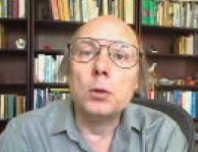
\includegraphics[width=0.3\columnwidth]{figs/figure2}
\end{center}

N.B. the tilde \verb|~| is an ``unsplittable'' space---it will never get
split across two different lines. This is useful before \verb|~\ref{...}|
and \verb|~\cite{...}|.

You need to add Bibtex references to \verb|references.bib|. Typical naming
convention is:
\begin{verbatim}
{Surname of first author}{Publication year}{First keyword of title}
\end{verbatim}
e.g. \verb|gu2015deep| for one of Ronghui's papers on deep specifications.
Then you can cite it with \verb|\cite{gu2015deep}|,
e.g.like this~\cite{gu2015deep}.
Make sure to use a \verb|~| before the citation.

I've defined a couple of comment macros in \verb|fastad-report.tex|.
\verb|\jhui{...}| will do this: \jhui{This is J-Hui's comment};
\verb|\jae{...}| will do this: \jae{This is James's comment}.
At the end, you can define these to become to be empty to quickly remove all
comments.
If you want to comment out a big block of text, just wrap them between
\verb|\if 0| and \verb|\fi|, like so (you cannot see what follows).
\if 0
C++ is not a programmer-friendly language.
\fi


\bibliographystyle{splncs04}
\bibliography{references}

\end{document}
